\documentclass{report}
\usepackage{graphicx}
\usepackage[utf8]{inputenc}
\usepackage[T1]{fontenc}   
\usepackage{geometry}       
\usepackage{hyperref}
\usepackage{float}

\title{\Huge Software Engineering Documentation \\[0.5cm]
        \Large Project: Blood Glucose Management Webapp}
\author{Fazion Pietro (VR501347) , Dal Degan Pietro (VR500305)}
\date{}

\begin{document}
\maketitle
\newpage
\tableofcontents
\newpage

\chapter{User Actions}

The developed Webapp serves three types of users:
\begin{itemize}
    \item Patient
    \item Doctor
    \item Admin
\end{itemize}
All user categories must authenticate to access their reserved area.
We will now look at the use cases and their sequence diagrams.
For clarity in visualizing the images, we will divide the use cases by user, although they are interconnected.

\section{Patient Use Cases}
\begin{figure}[H]
    \centering
    
\includegraphics[width=\textwidth, height=\textheight, keepaspectratio]
    {img/Use_case/Use_case_paziente.png}
\end{figure}

After authenticating, the patient is redirected to their homepage, where they will find:
\begin{itemize}
    \item A chart showing their blood glucose trends over time
    \item A button to insert blood glucose readings
    \item The latest recorded blood glucose entries
    \item A form for communicating symptoms and diseases
    \item An area to mark taken medications
    \item A form to contact the doctor
\end{itemize}

\vspace{1cm}
We now list the use cases shown in the image below:
\begin{itemize}
    \item Insert blood glucose reading
    \item Report pathologies, diseases, and/or symptoms to the doctor
    \item Daily recording of taken medications
    \item Contact the doctor
\end{itemize}

\subsection{Insert Blood Glucose Reading}
The patient must be able to insert their glycemic level. By clicking the "insert glucose" button, a modal appears where they can input their glycemic level. Specifically, when a patient inserts a reading that falls outside the normal range (80-130 mg/dL and maximum 180mg/dL after meals), the system records the reading and generates an alert to inform the doctor.

\fbox{
    \begin{minipage}{0.9\textwidth}
        \textbf{Actors: } Patient \\
        \textbf{Preconditions: } The patient must be authenticated \\
        \textbf{Steps: }
        \begin{enumerate}
            \item The patient clicks the "New reading" button
            \item The patient fills the glucose modal field that appears
            \item The patient clicks the "send" button
            \item The validity of the entered data is checked
            \item Alerts for Doctor and Patient may be created in case of out-of-range values
        \end{enumerate}
        \textbf{Postconditions: } The glycemic data is inserted into the database
    \end{minipage}
}
\begin{figure}[H]
    \centering
    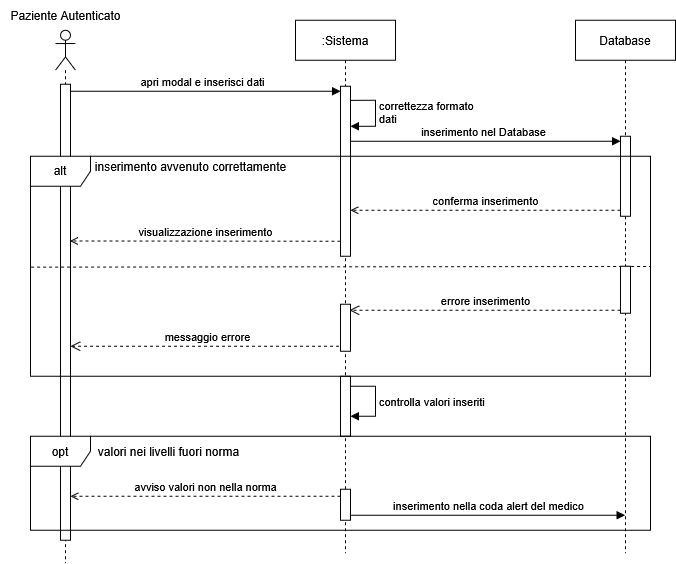
\includegraphics[width=\linewidth, height=0.5\textheight, keepaspectratio]
    {img/Use_case/Inserimento_glicemia.png}
\end{figure}

\subsection{Reporting Pathologies, Diseases, and/or Symptoms}
The patient can report any pathologies, diseases, and/or symptoms to their doctor. In the dedicated box, the patient can select various symptoms from checkboxes or type them freely in the text field along with any diseases and pathologies.

\fbox{
    \begin{minipage}{0.9\textwidth}
        \textbf{Actors: } Patient \\
        \textbf{Preconditions: } The patient must be authenticated \\
        \textbf{Steps: }
        \begin{enumerate}
            \item The patient selects the checkboxes for the experienced symptoms
            \item The patient fills in the text field with pathologies and diseases
            \item The patient clicks the "send report" button
            \item The report is communicated to the doctor
        \end{enumerate}
        \textbf{Postconditions: } The report is inserted into the database and notified to the doctor
    \end{minipage}
}

\begin{figure}[H]
    \centering
    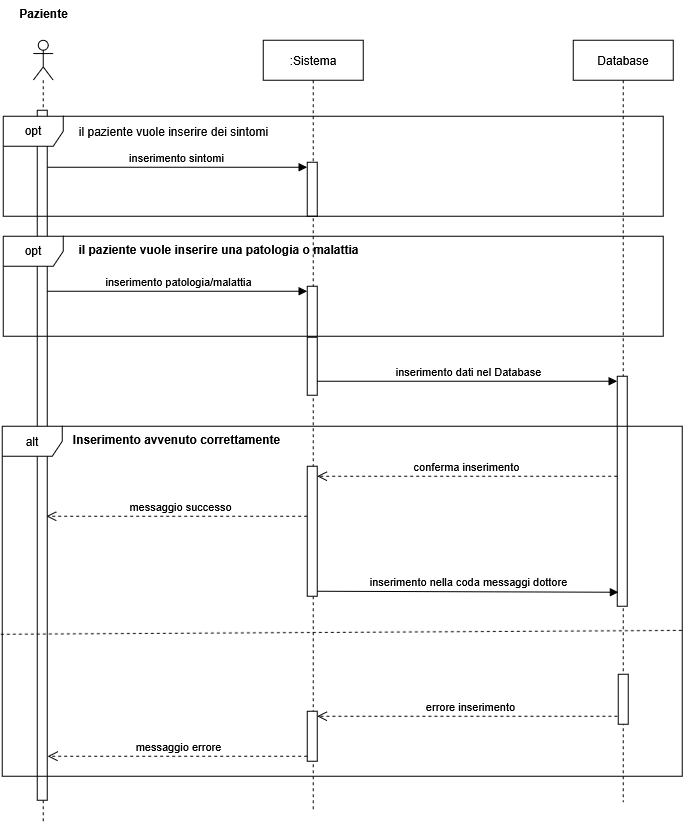
\includegraphics[width=\linewidth, height=0.55\textheight, keepaspectratio]
    {img/Use_case/Segnala_medico.png}
\end{figure}

\subsection{Daily Recording of Taken Medications}
The patient can record their daily taken medications. In the appropriate box, there will be the list of medications the patient should take during the day; they simply need to select the taken ones and press the "send report to doctor" button so they can be recorded.

\fbox{
    \begin{minipage}{0.9\textwidth}
        \textbf{Actors: } Patient \\
        \textbf{Preconditions: } The patient must be authenticated \\
        \textbf{Steps: }
        \begin{enumerate}
            \item The patient selects the taken medications from the list
            \item The patient clicks the "send report to doctor" button
            \item The entered data is then checked
            \item Registration confirmation is provided
        \end{enumerate}
        \textbf{Postconditions: } The taken medications are recorded in the database
    \end{minipage}
}

\begin{figure}[H]
    \centering
    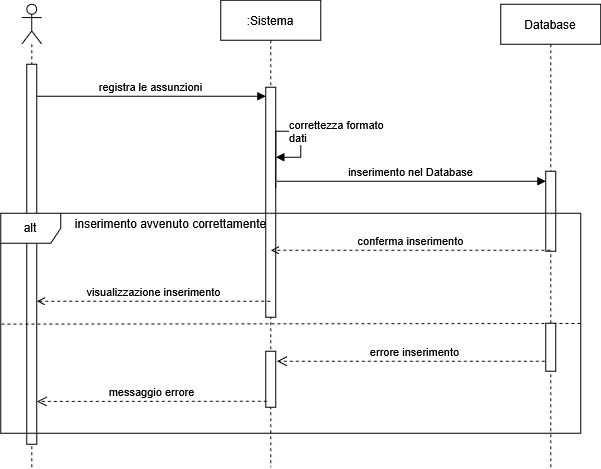
\includegraphics[width=\linewidth, height=0.55\textheight, keepaspectratio]
    {img/Use_case/Medicinali_assunti.png}
\end{figure}

\subsection{Contact the Doctor}
The Patient can contact their doctor using a dedicated form. In the appropriate box, the patient must fill out the text field and select the message priority among low, medium, and high; then press "send" to send the message.

\begin{figure}[H]
    \centering
    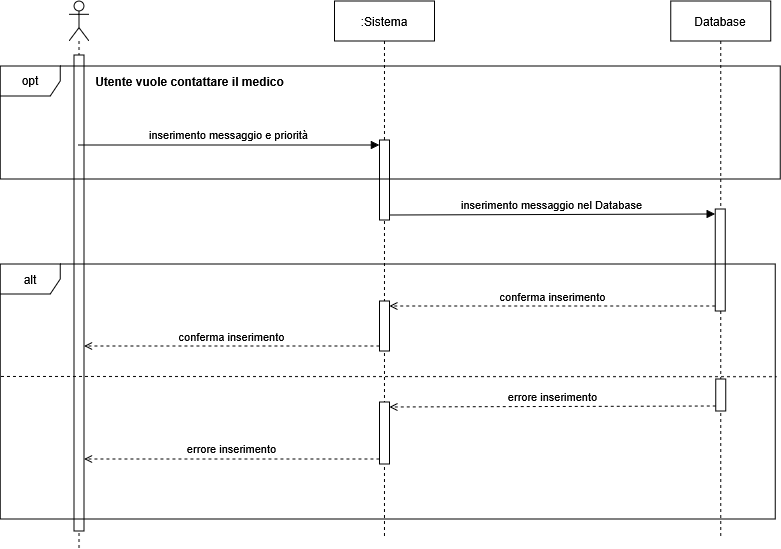
\includegraphics[width=\textwidth, height=\textheight, keepaspectratio]
    {img/Use_case/Contatta_medico.png}
\end{figure}

\section{Doctor Use Cases}
\begin{figure}[H]
    \centering
    
\includegraphics[width=\textwidth, height=\textheight, keepaspectratio]
    {img/Use_case/Use_case_medico.png}
\end{figure}

After authenticating, the doctor is redirected to their homepage, where they will find:
\begin{itemize}
    \item A box with the list of received messages and alerts
    \item An area for managing patient therapies
    \item An area for managing patients
\end{itemize}

\subsection{View Alerts for the Doctor}
The doctor will have the list of messages and alerts on the right side of their homepage; when they have read the alert, they can press "read" to mark it and remove it.

\begin{figure}[H]
    \centering
    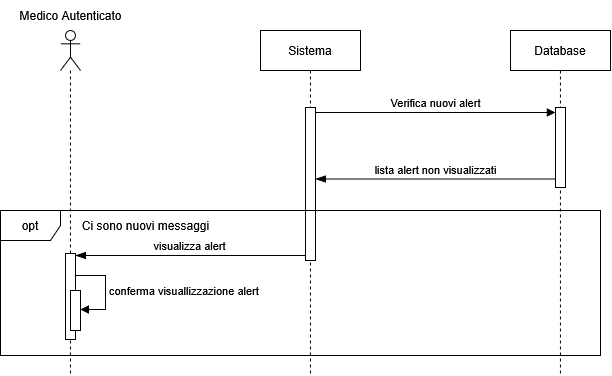
\includegraphics[width=\textwidth, height=\textheight, keepaspectratio]
    {img/Use_case/Vis_alert_medico.png}
\end{figure}

\subsection{Therapy Management}
The doctor can modify a therapy by clicking the pencil button next to it, delete it using the trash can button, or create a new one using the "New Therapy" button.

\begin{figure}[H]
    \centering
    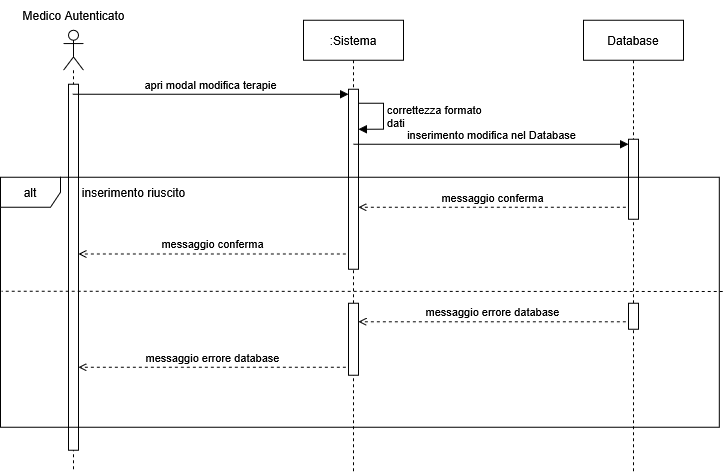
\includegraphics[width=\linewidth, height=\textheight, keepaspectratio]
    {img/Use_case/Modifica_terapie.png}
\end{figure}
\begin{figure}[H]
    \centering
    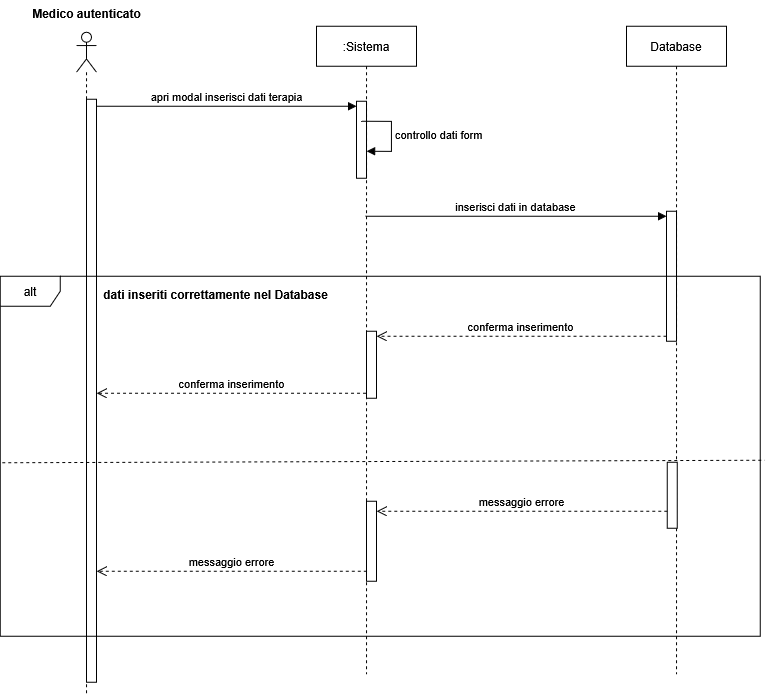
\includegraphics[width=\linewidth, height=\textheight, keepaspectratio]
    {img/Use_case/Crea_terapie.png}
\end{figure}
\begin{figure}[H]
    \centering
    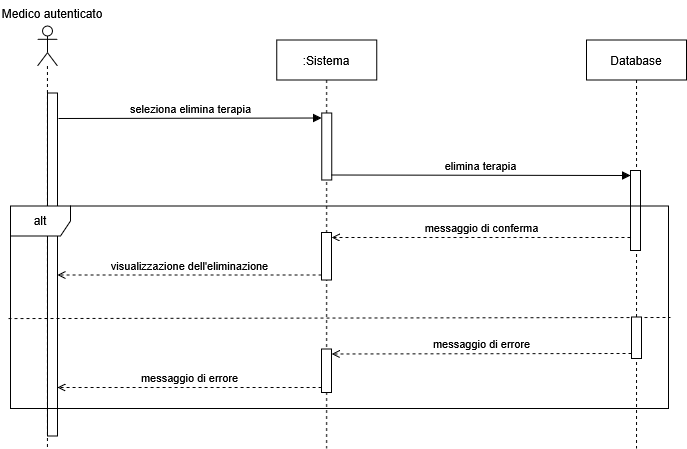
\includegraphics[width=\linewidth, height=\textheight, keepaspectratio]
    {img/Use_case/Elimina_terapie.png}
\end{figure}

\subsection{Patient Management}
The doctor can decide to edit a Patient's information, delete it, or view the glycemic trend details using the respective icons.

\begin{figure}[H]
    \centering
    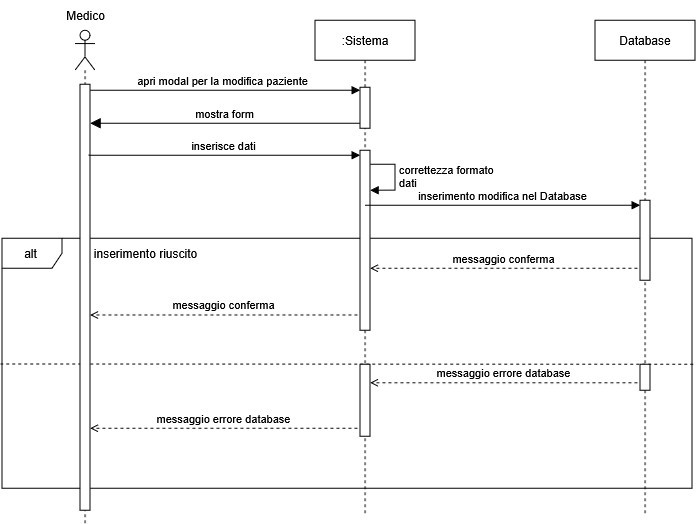
\includegraphics[width=\textwidth, height=0.5\textheight, keepaspectratio]
    {img/Use_case/Modifica_paziente.png}
\end{figure}
\begin{figure}[H]
    \centering
    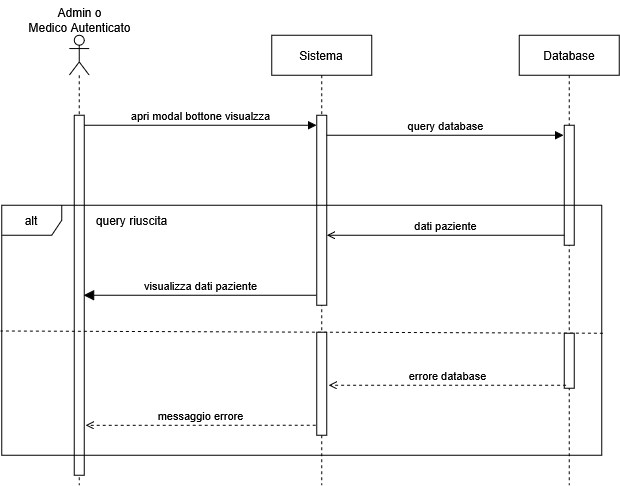
\includegraphics[width=\textwidth, height=\textheight, keepaspectratio]
    {img/Use_case/Visualizza_paziente.png}
\end{figure}
\begin{figure}[H]
    \centering
    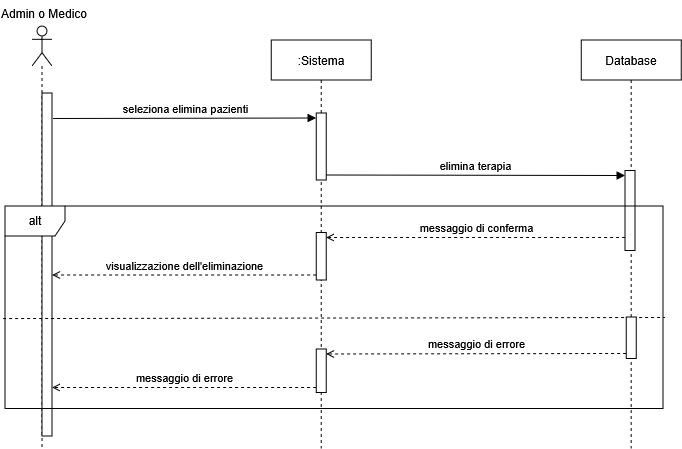
\includegraphics[width=\textwidth, height=\textheight, keepaspectratio]
    {img/Use_case/Elimina_pazienti.png}
\end{figure}

\section{Admin Use Cases}
\begin{figure}[H]
    \centering
    
\includegraphics[width=\textwidth, height=\textheight, keepaspectratio]
    {img/Use_case/Use_case_admin.png}
\end{figure}

After authenticating, the admin is redirected to their homepage, where they will find features to manage users (Doctors and Patients) and view system logs.

\begin{figure}[H]
    \centering
    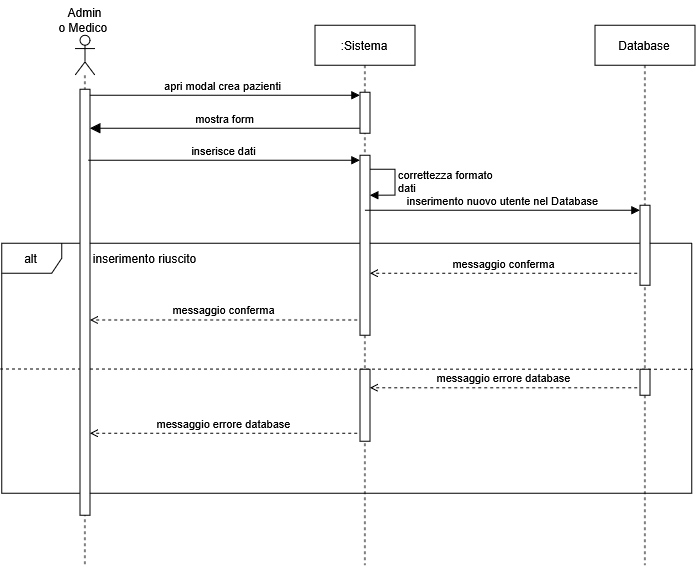
\includegraphics[width=\textwidth, height=\textheight, keepaspectratio]
    {img/Use_case/Crea_paziente.png}
\end{figure}
\begin{figure}[H]
    \centering
    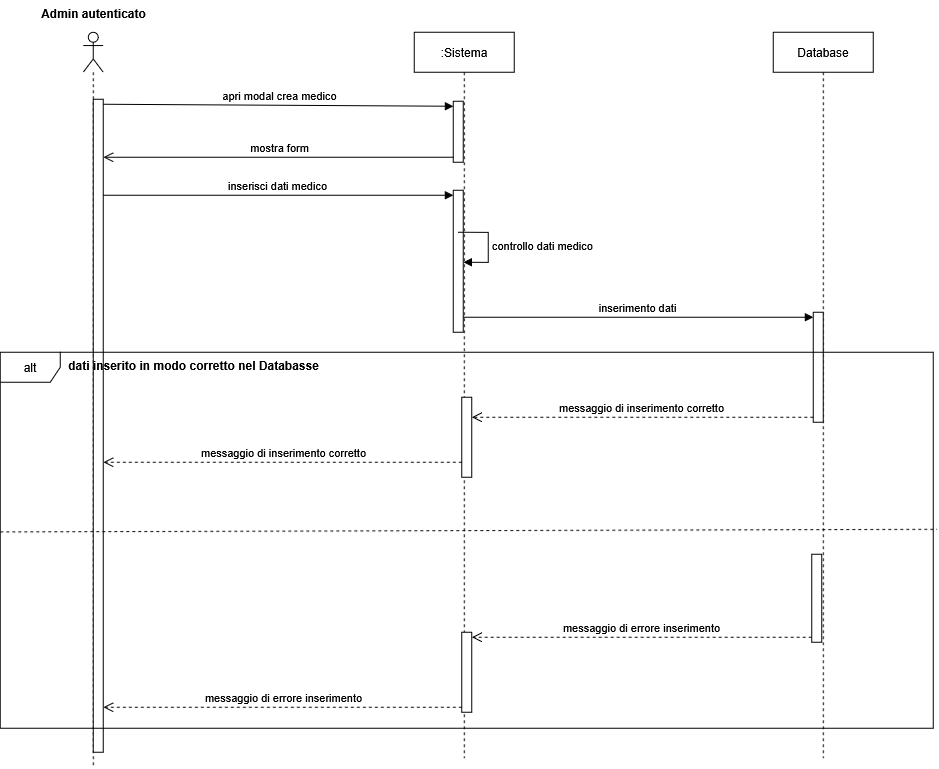
\includegraphics[width=\textwidth, height=\textheight, keepaspectratio]
    {img/Use_case/Crea_medico.png}
\end{figure}

\chapter{Activity Diagrams}

\section{Authentication Diagram}
\begin{figure}[H]
    \centering
    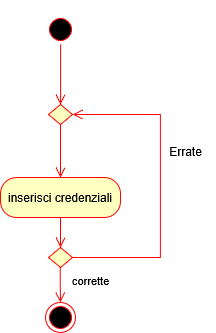
\includegraphics[width=\textwidth, height=0.5\textheight, keepaspectratio]
    {img/Diagrammi/DA_autenticazione.png}
\end{figure}

\section{Patient Diagram}
\begin{figure}[H]
    \centering
    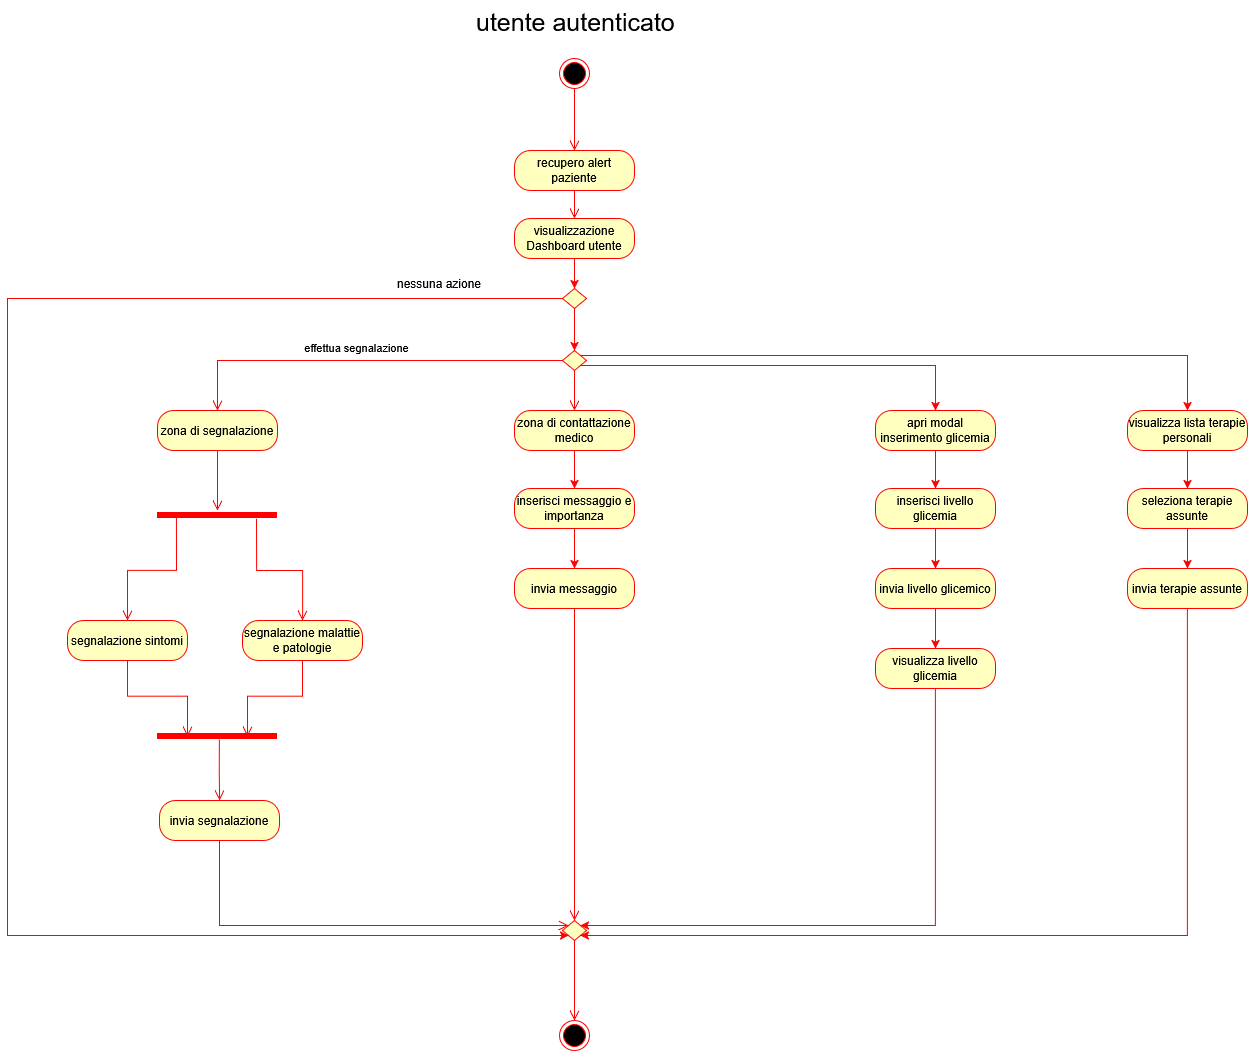
\includegraphics[width=\textwidth, height=\textheight, keepaspectratio]
    {img/Diagrammi/DA_paziente.png}
\end{figure}

\section{Doctor Diagram}
\begin{figure}[H]
    \centering
    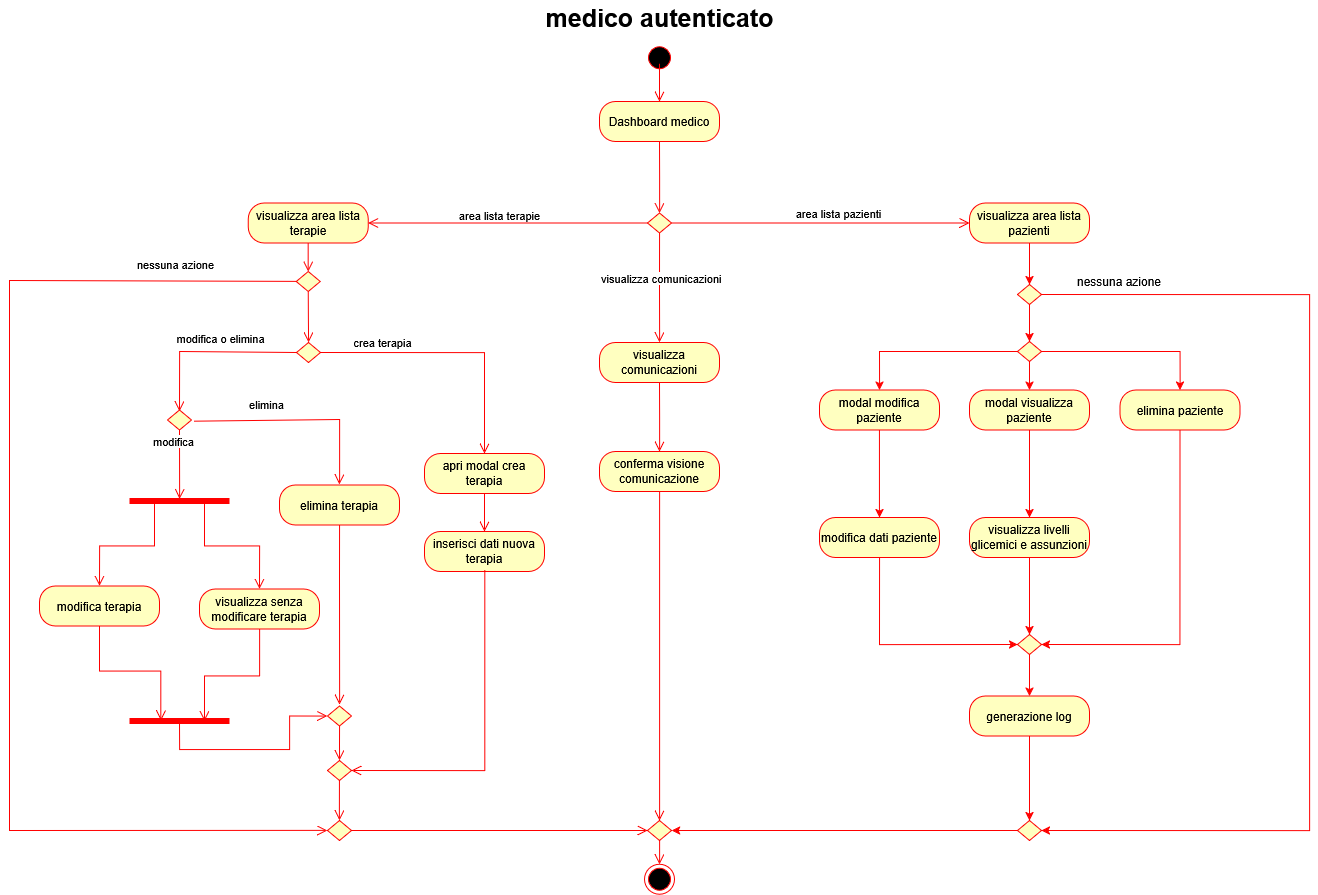
\includegraphics[width=\textwidth, height=\textheight, keepaspectratio]
    {img/Diagrammi/DA_medico.png}
\end{figure}

\section{Admin Diagram}
\begin{figure}[H]
    \centering
    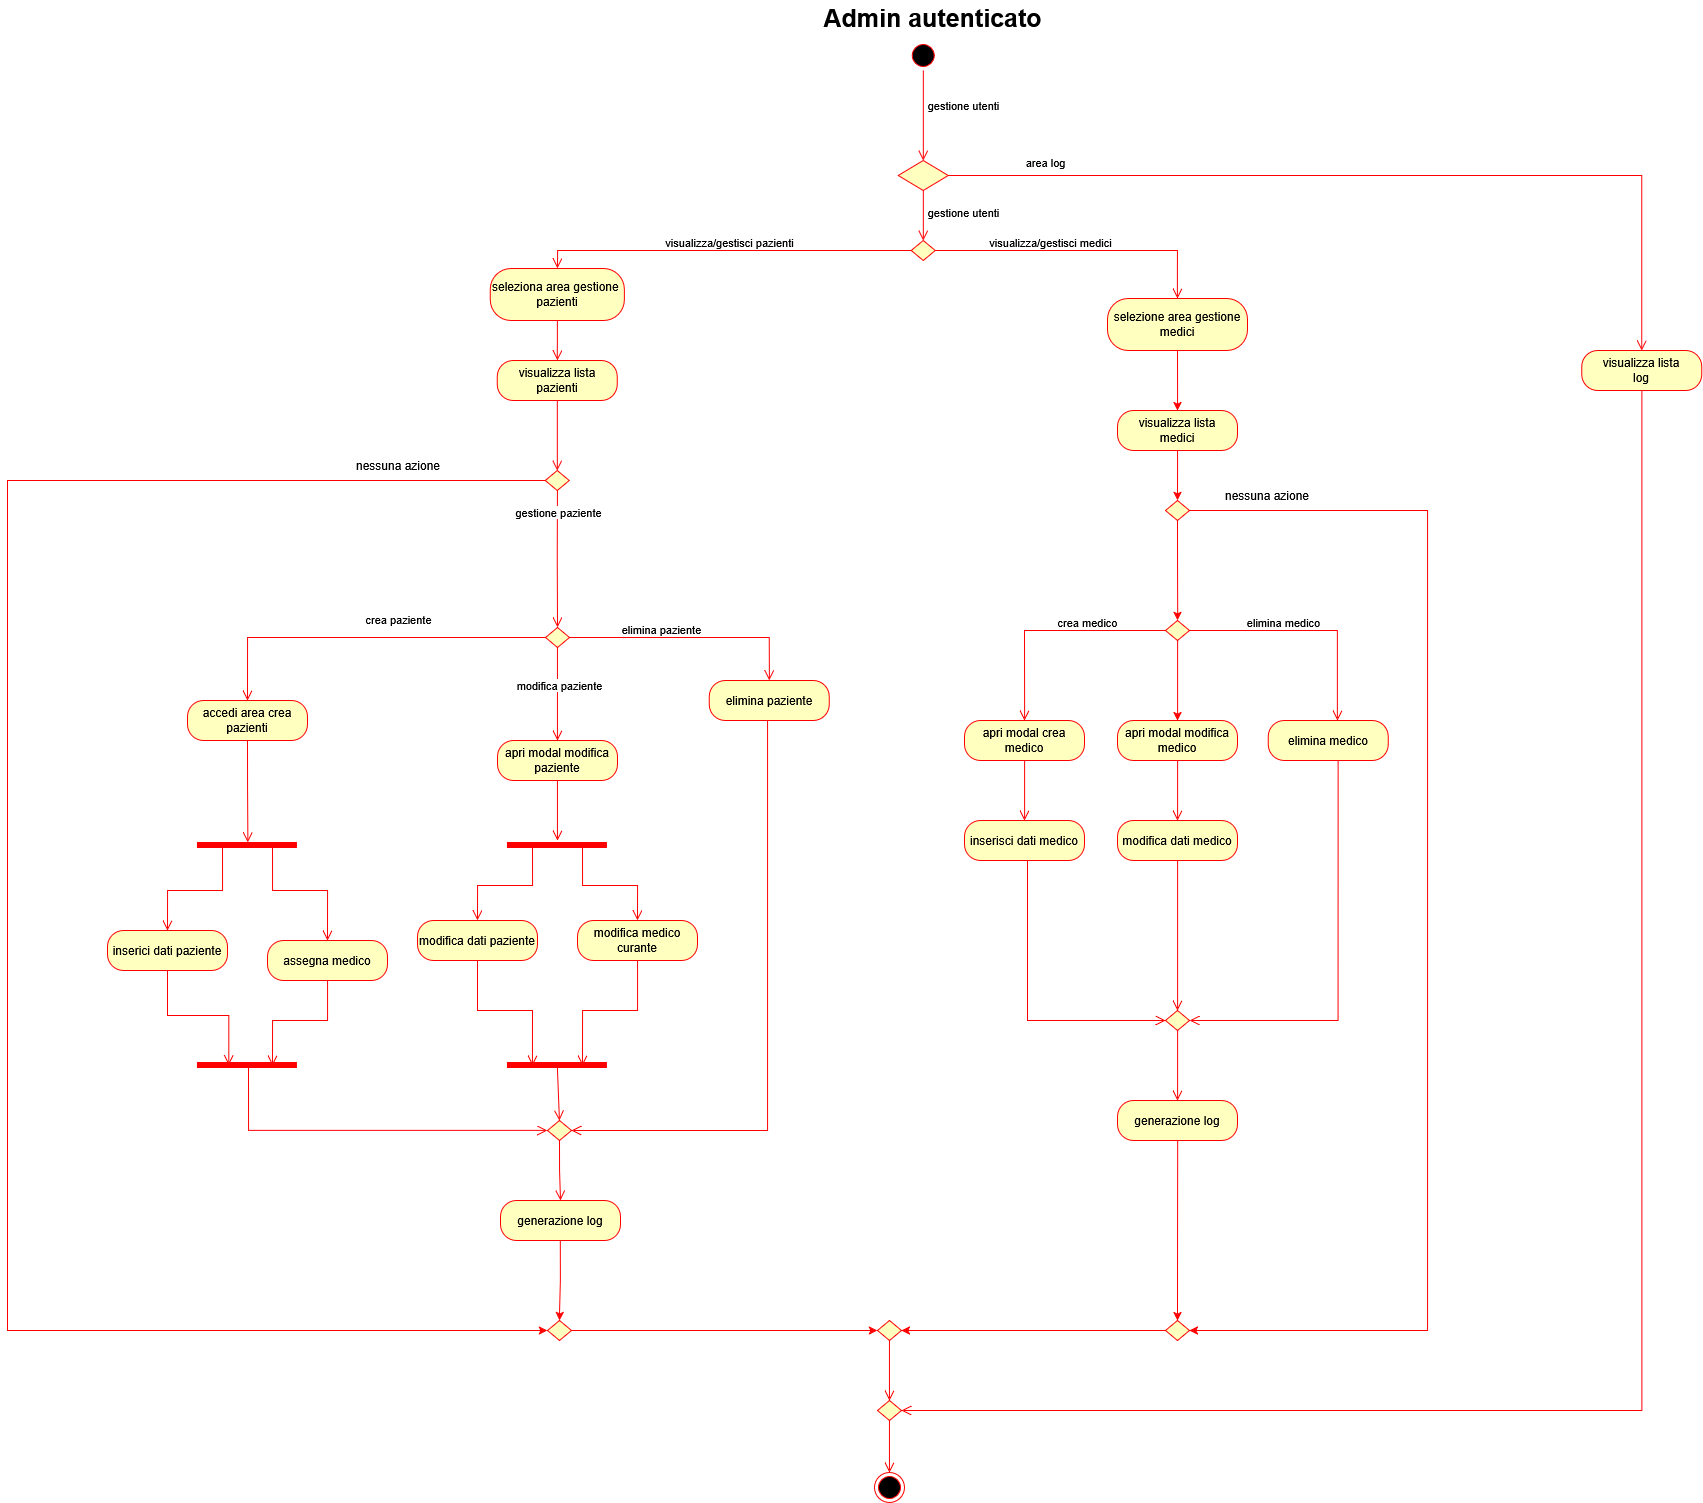
\includegraphics[width=\textwidth, height=\textheight, keepaspectratio]
    {img/Diagrammi/DA_admin.png}
\end{figure}

\chapter{UML Diagrams}

\section{Class Diagram - Entity Package}
\begin{figure}[H]
    \centering
    
\includegraphics[width=0.98\textwidth, keepaspectratio]
    {img/UML/entity_class_diagram.png}
    \caption{Class Diagram - Entity Package}
\end{figure}

The \texttt{entity} package defines the object representation of the data schema, including entities like Utente, Paziente, Terapia, Assunzione, Rilevazione, Comunicazione, Log, and BlacklistedToken.

\section{UML Sequence Diagrams}

\subsection{Authentication (Sign-In)}
\begin{figure}[H]
    \centering
    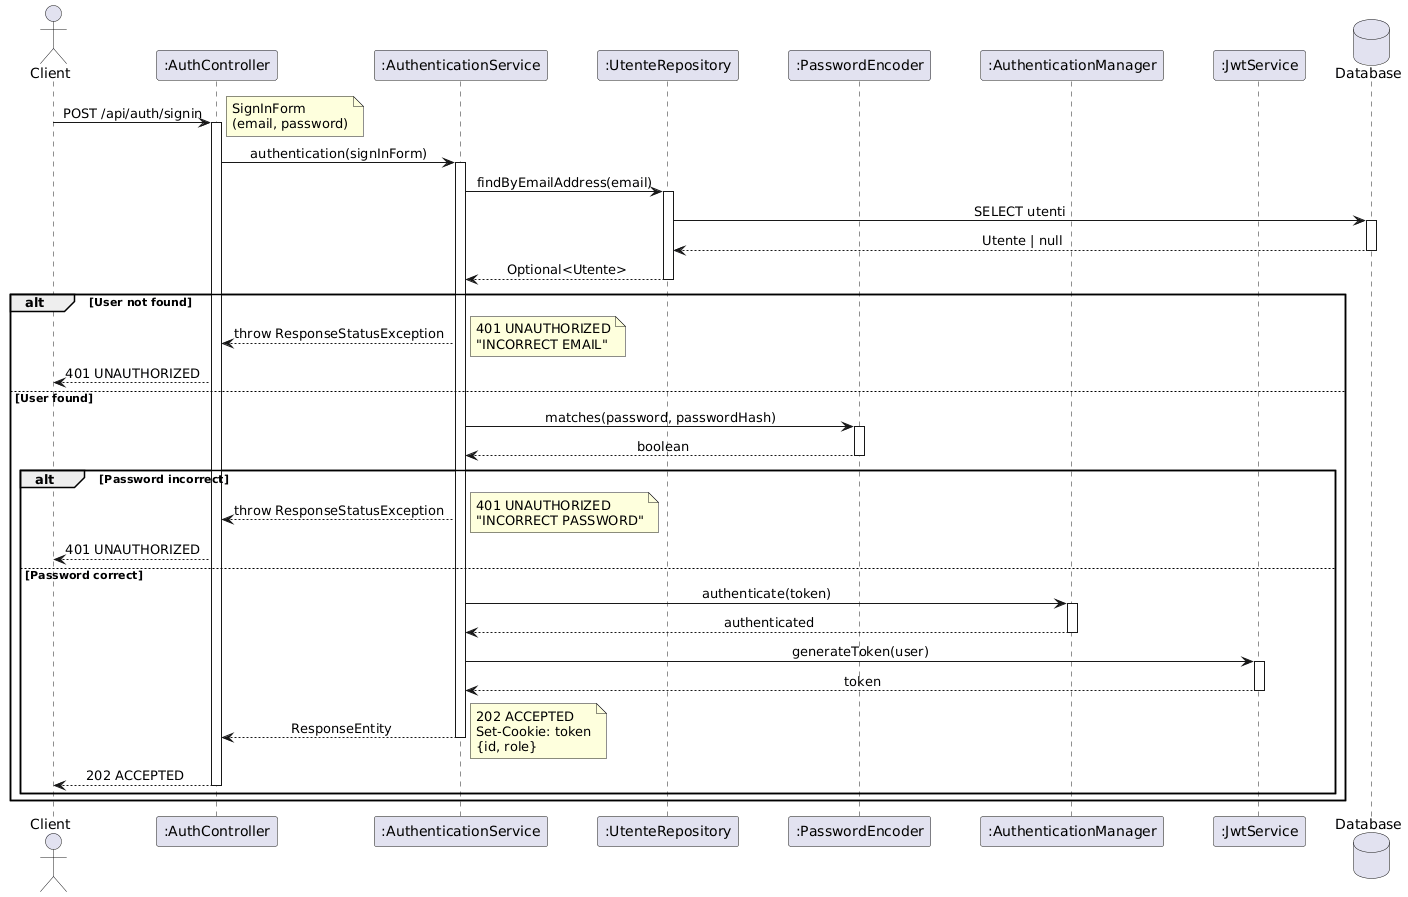
\includegraphics[width=\textwidth, keepaspectratio]
    {img/UML/sequence_authentication.png}
\end{figure}

\subsection{User Registration}
\begin{figure}[H]
    \centering
    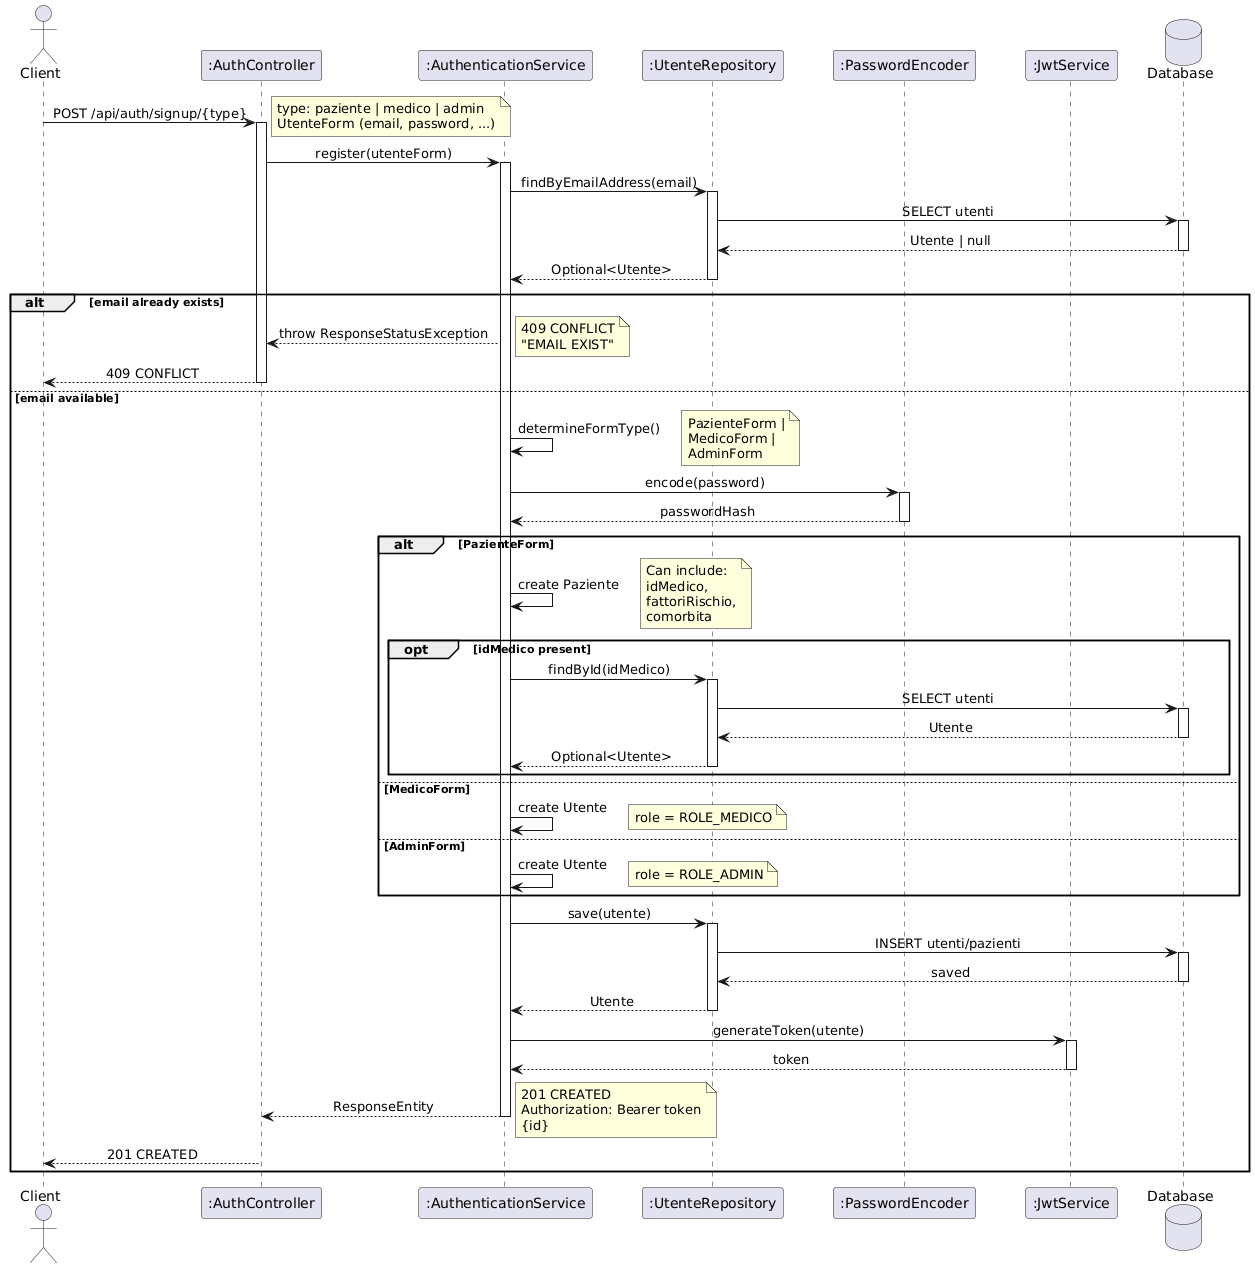
\includegraphics[width=\textwidth, keepaspectratio]
    {img/UML/sequence_registration.png}
\end{figure}

\subsection{Therapy Creation}
\begin{figure}[H]
    \centering
    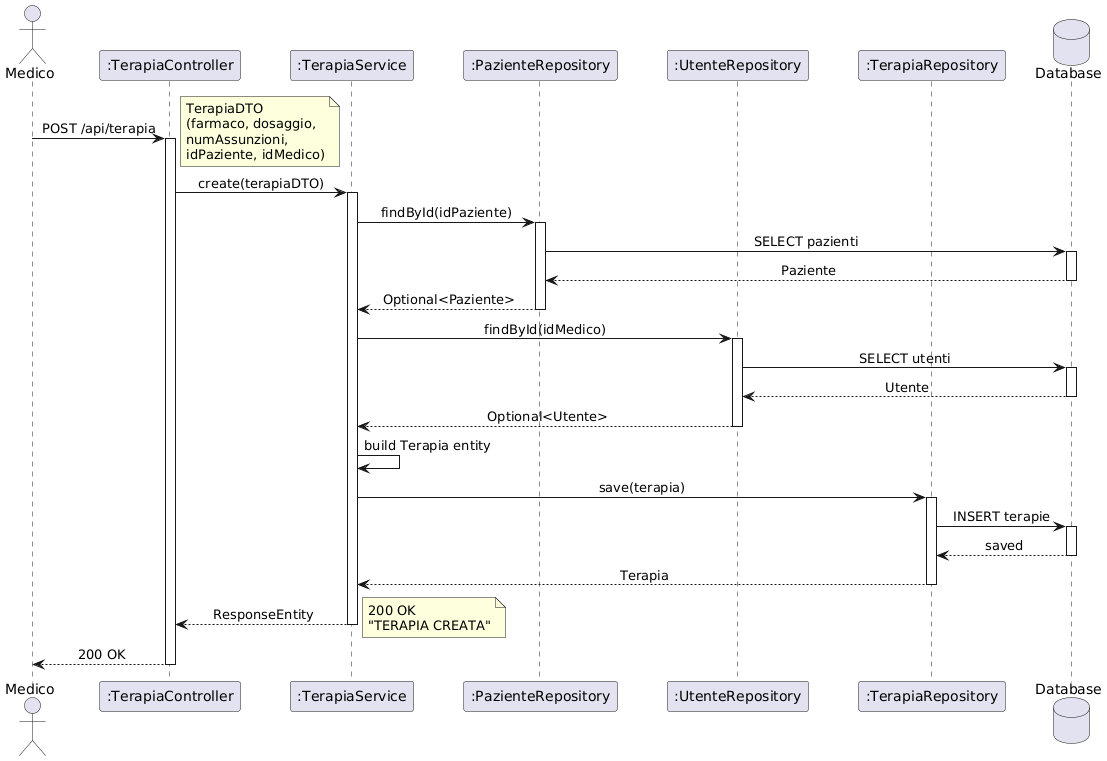
\includegraphics[width=0.9\textwidth, keepaspectratio]
    {img/UML/sequence_create_terapia.png}
\end{figure}

\subsection{Add Reading with Automatic Alert}
\begin{figure}[H]
    \centering
    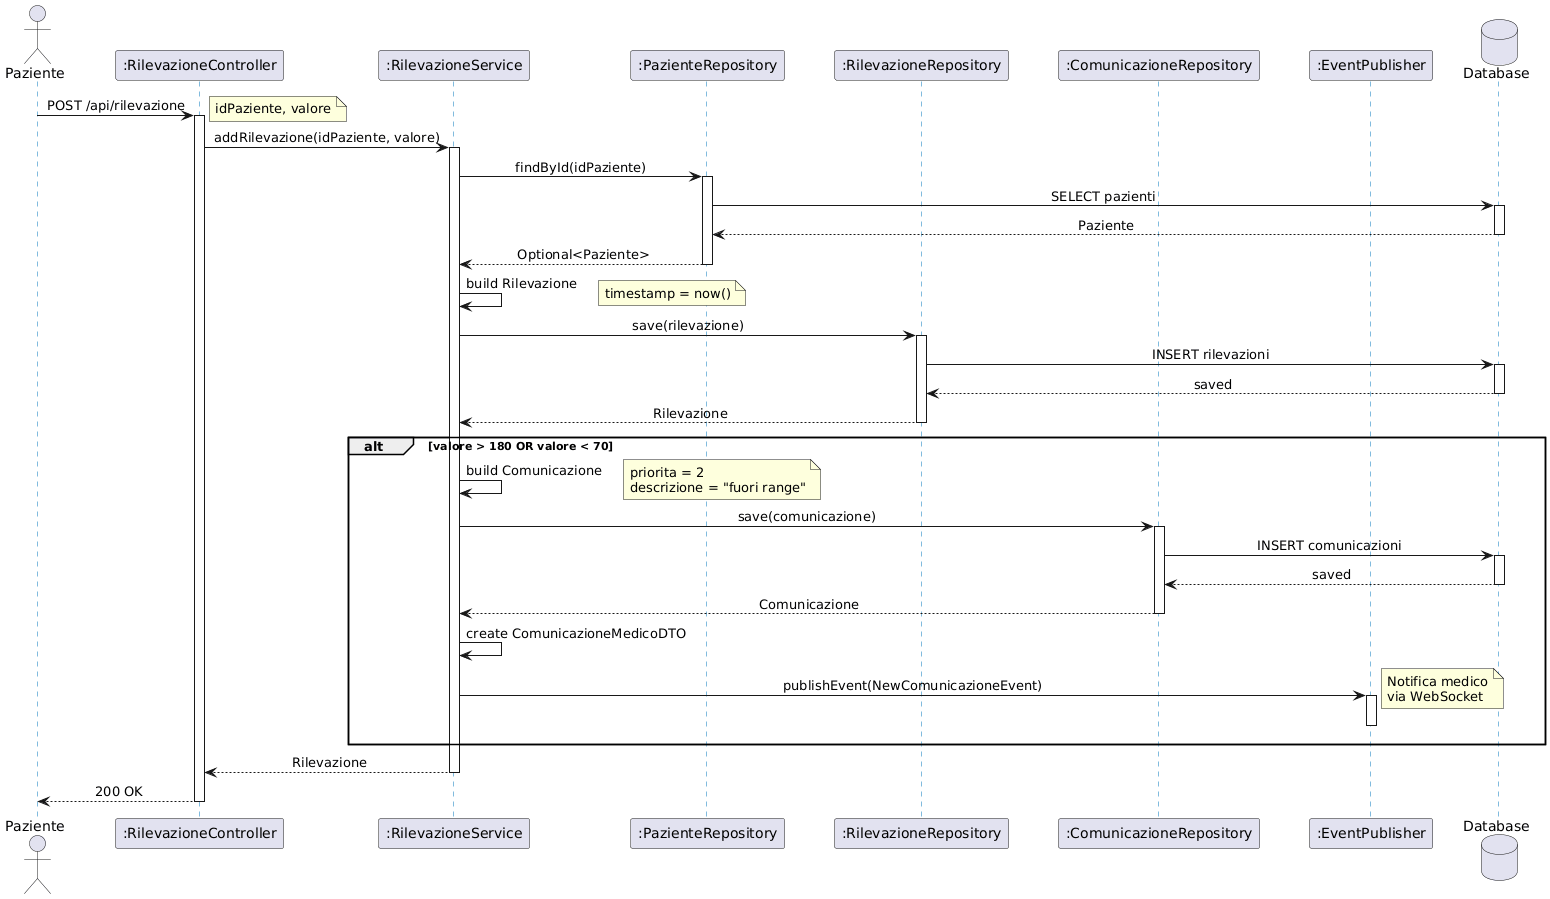
\includegraphics[width=0.9\textwidth, keepaspectratio]
    {img/UML/sequence_add_rilevazione.png}
\end{figure}

\subsection{JWT Filter for Request Authentication}
\begin{figure}[H]
    \centering
    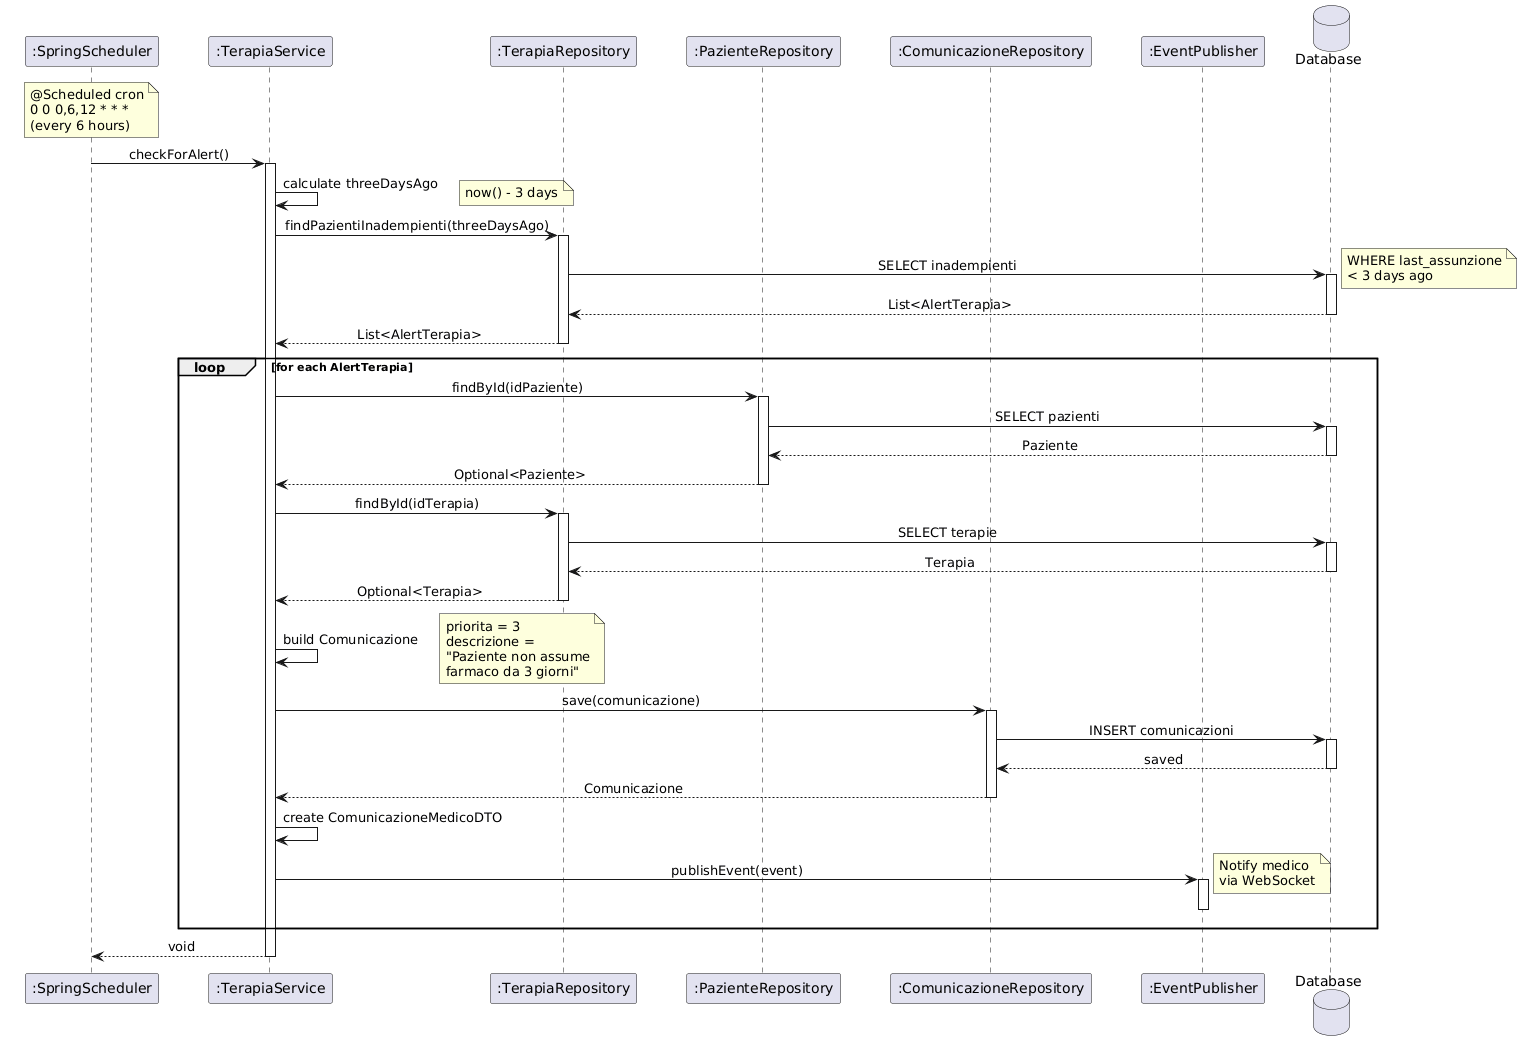
\includegraphics[width=0.9\textwidth, keepaspectratio]
    {img/UML/sequence_jwt_filter.png}
\end{figure}

\subsection{Logout}
\begin{figure}[H]
    \centering
    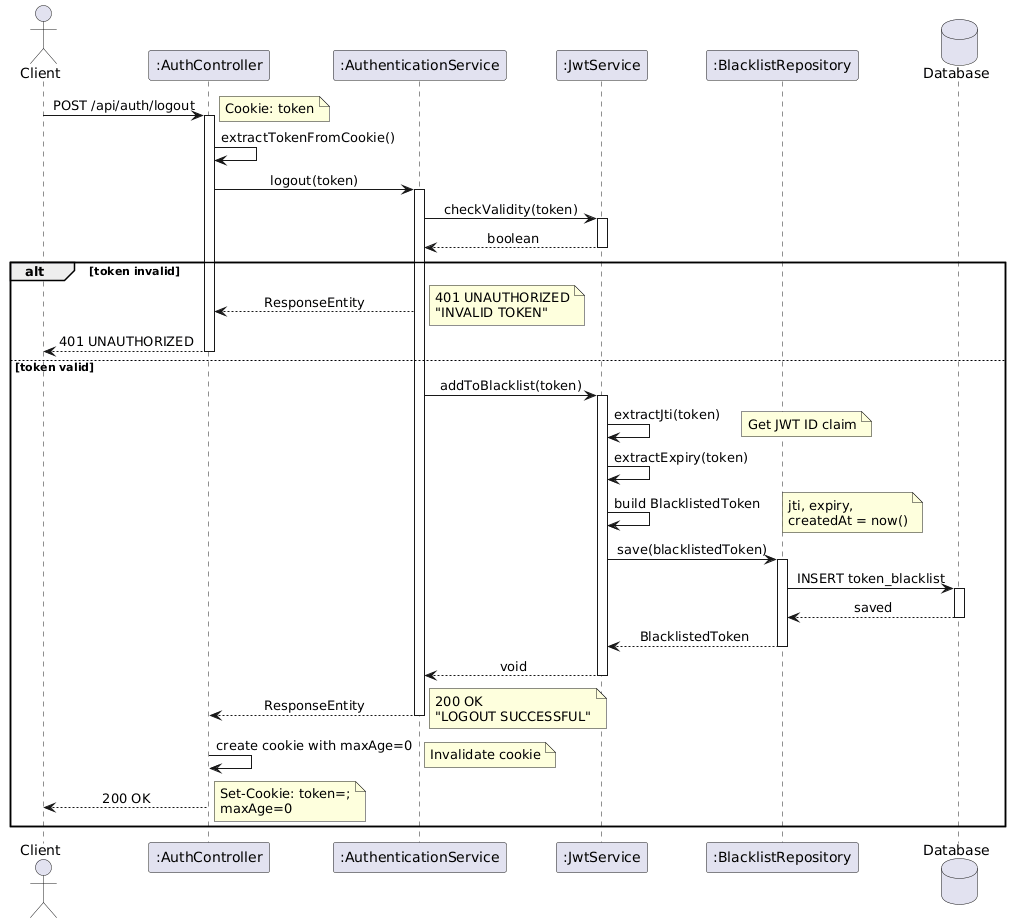
\includegraphics[width=\textwidth, keepaspectratio]
    {img/UML/sequence_logout.png}
\end{figure}

\subsection{Scheduled Automatic Therapy Check}
\begin{figure}[H]
    \centering
    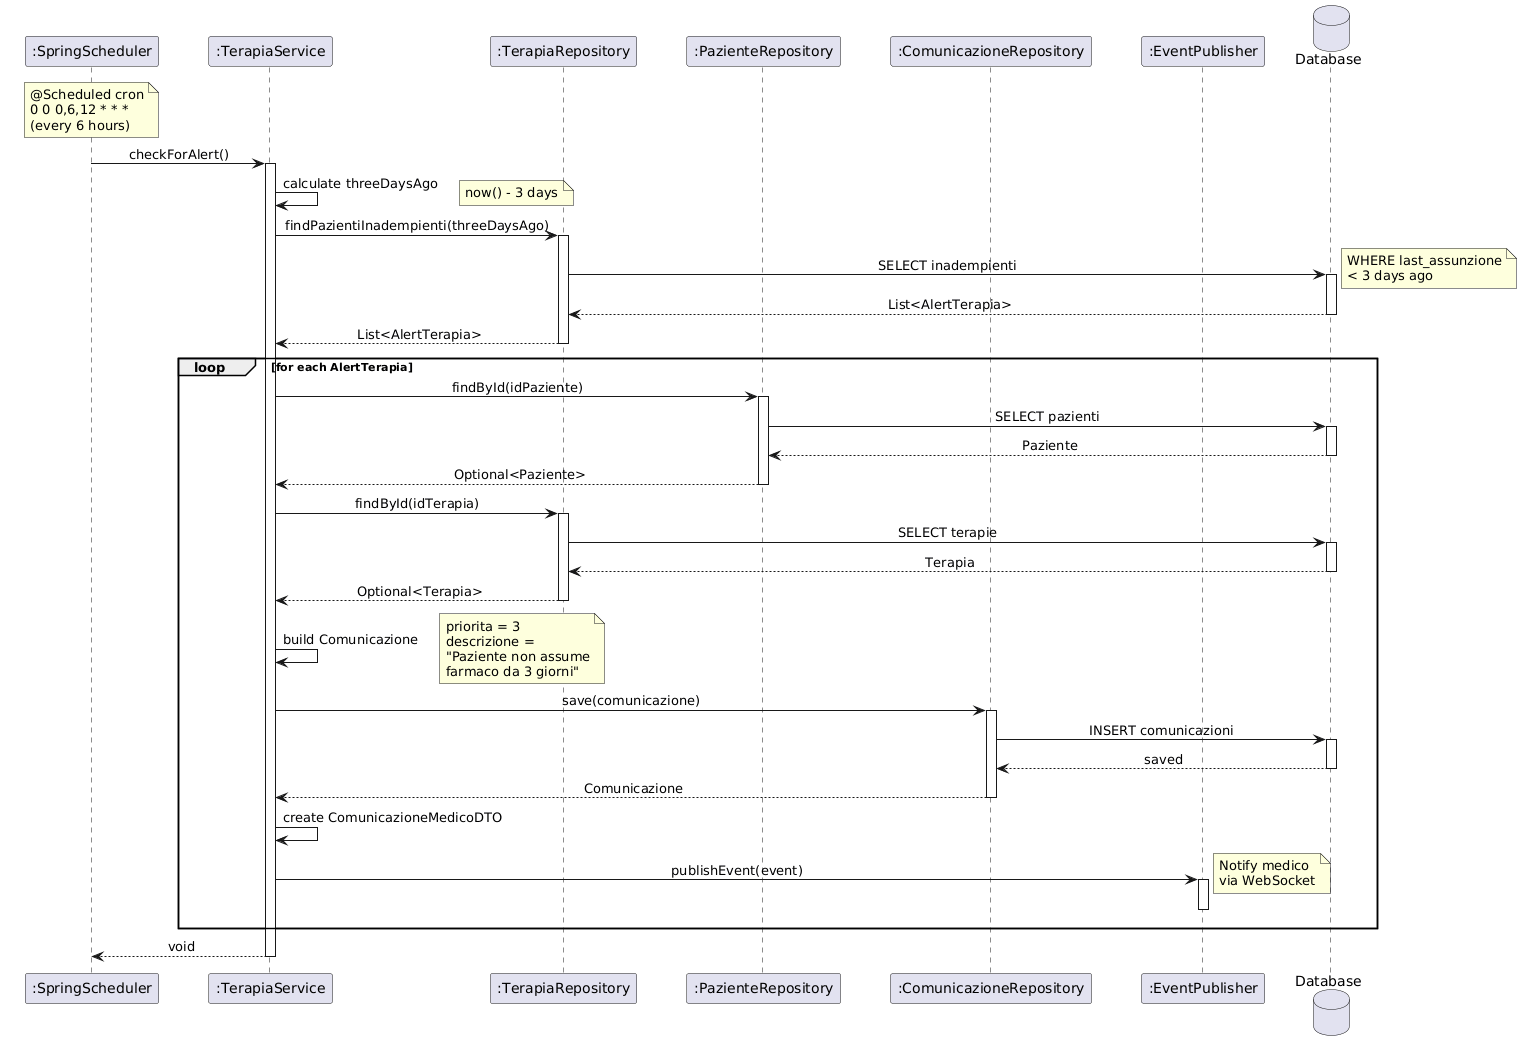
\includegraphics[width=0.9\textwidth, keepaspectratio]
    {img/UML/sequence_scheduled_therapy_check.png}
\end{figure}

\chapter{Software Development}
\section{Development Methodology}
An iterative and incremental Agile-based process model was adopted for the system development, characterized by high operational flexibility depending on project specificities. The process includes Requirement Analysis, Sprint planning, Implementation, Testing, and Documentation updates.

\begin{figure}[H]
    \centering
    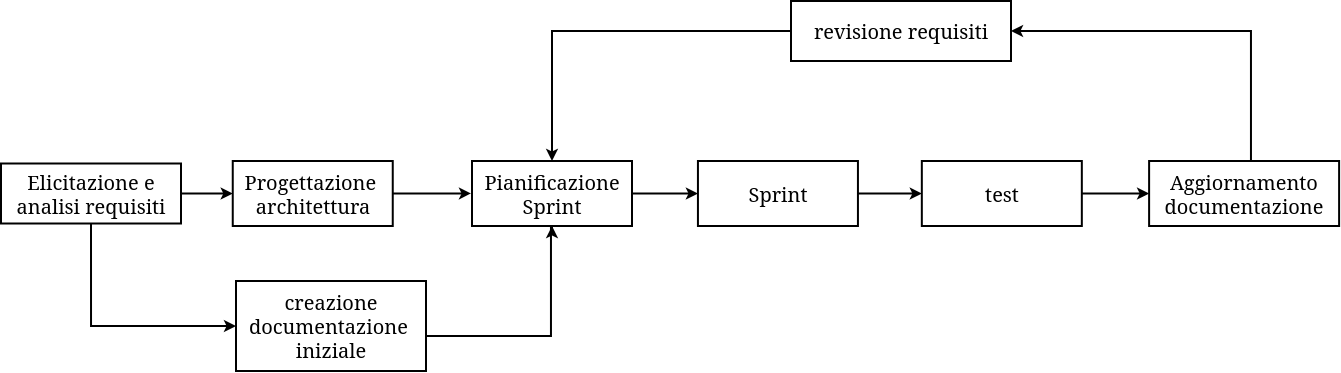
\includegraphics[width=\textwidth, height=\textheight, keepaspectratio]
    {img/Diagrammi/ProcessoSviluppo_tmp.png}
\end{figure}

\section{Architecture}
The software adopts a \textit{Client-Server} architecture with elements of the \textit{Model-View-Controller} pattern.
\begin{figure}[H]
    \centering
    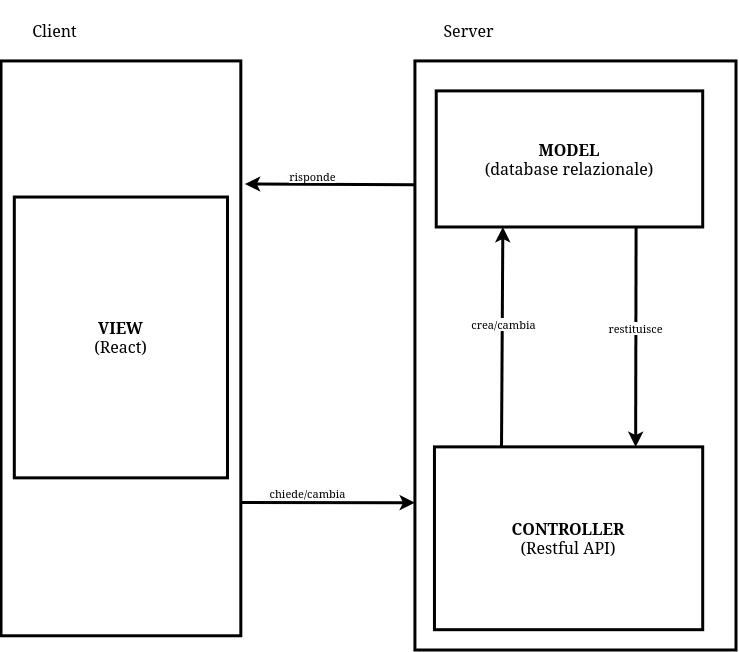
\includegraphics[width=0.7\textwidth, height=\textheight, keepaspectratio]
    {img/Diagrammi/architettura.png}
\end{figure}

\section{Implementation}
Backend (Spring Boot) is structured into Entity, Repository, Service, Controller, DTO, Config, Filter, and Exception packages. The Frontend is developed with React 18 and TypeScript.

\chapter{Testing}
Automated testing was performed using JUnit and Mockito to verify the correct functioning of services. Manual tests and external user tests were also conducted to ensure usability and correct operation of the system.

\end{document}
